\section{Introduction}
\label{sec:introduction}

Misconfiguration of security and networking devices is a source of
  vulnerabilities for various commercial and private network.
  System administrators cannot be solely be held responsible for such
  misconfiguration. Commercial networking and security device manufacturers have their own
  syntax for management and configuration. Some, such as CISCO IOS,
  have become de facto standards which are `` adhered to '' by other vendors.
  However, broadly speaking, there is no standard syntax for router and 
  firewall configuration.   This complicates the configuration tasks for system administrators,
  who deploy such devices in large corporates.The system administrator (s) need to be
  familiar with the language peculiarities of various   configuration interfaces, increasing 
  the chances of misconfiguration and introducing redundant and ineffective routing and firewalling
  policies. A common vulnerabilty in firewalling configuration arises due to the order in which the 
  semantic analyzer analyzes the rules. Firewall configurations may be as simple 
  as packet filtering rules; maybe much more complex such for stateful firewalling,
  protocol specific vulnerability detection and deep packet inspection.
  Certain firewalls match the incoming packets to the first matched rule
  while the others match the last one.The absence of any particular firewall and router configuration
  language motivates us to design {\bf LANCOM} ({\bf LA}nguage for {\bf N}etwork {\bf CO}nfiguration and
  {\bf M}anagement). We plan to design, implement and test LANCOM with the following objectives:

  \begin{enumerate}
    \item `` Device manufacturer independent '' description of firewalling and
             routing configuration. 
    \item  Separation between network topology and
           firewalling policy description.We intend to achieve this using 
           {\it role - based} policy description. 
  \end{enumerate}

Following figure ~ \ref {fig:block_dgm} presents a rudimentary description of 
the language compiler can and how it can be used to generate vendor specific 
 routing and firewalling configuration scripts. 

\begin{figure}[ht] 
\label {fig:block_dgm}

%\centering 
\begin{center}
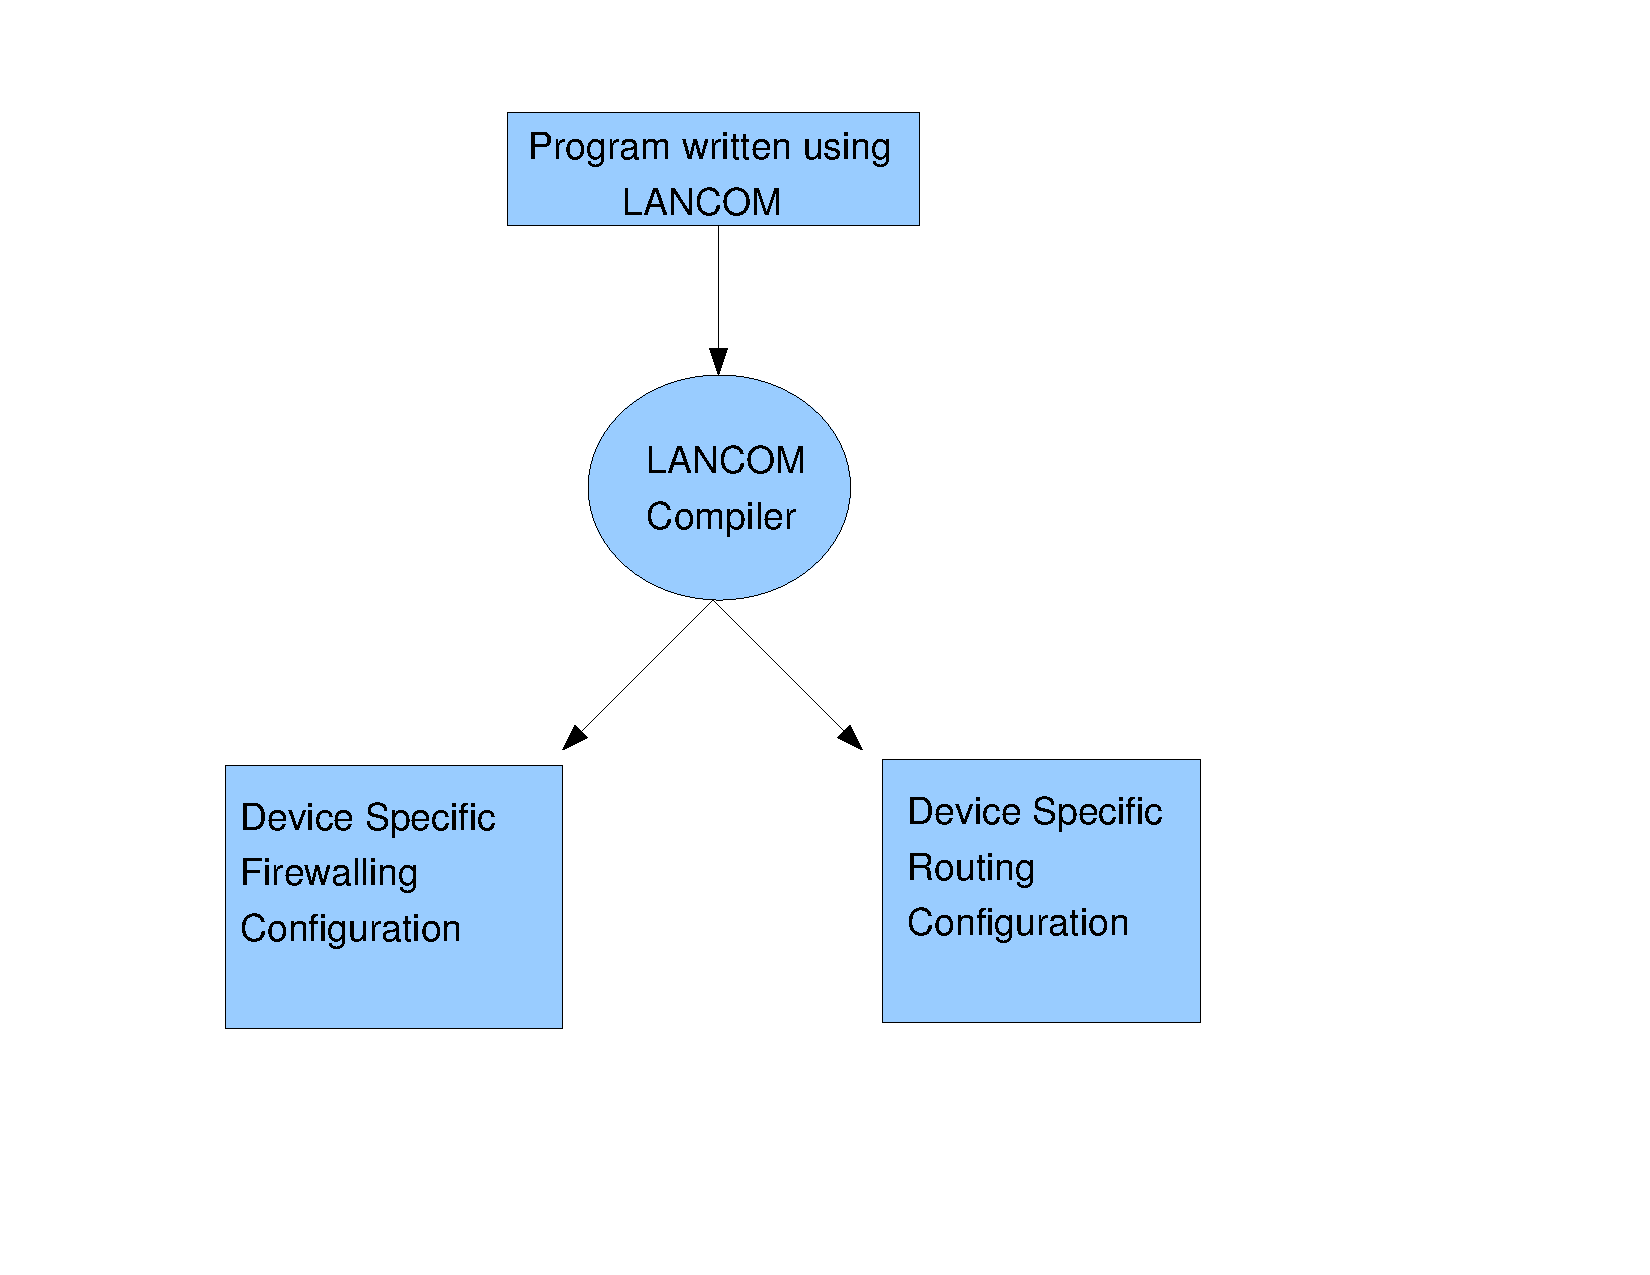
\includegraphics[scale=0.35]{figs/language_blk_dgm.pdf}
\end{center}
\smallcaption {The LANCOM Compiler Generates Output Specific to the Firewall / Router}
 \end{figure}
